\chapter{Formal semantics of Ravenscar}{``The essence of
  mathematics is not to make simple things\\complicated, but to make
  complicated things simple''}{Stanley Gudder}
\label{chap:formal_sem}

The previous chapters presented the rules for code generation from
AADL system models, as well as constructs for deterministic real-time
connectors for control system development. This chapter presents a
static semantics for the code that is generated, which is a subset of
Ada Ravenscar. Also presented is a structured operational semantics
that captures the dynamic evolution of the generated system. This
semantics is the basis for on-going developments targeted at enhancing
the tool-chain with simulation and verification features.

Formal semantics of any system describe its behavior in unambiguous
terms. For programming languages, the semantics can be given in many
different methods and formalisms. The method of assigning meanings to
programs, however, falls in one of three main classes:\\

\begin{description}
\item[Denotational:]{Each statement or instruction in the language
  being considered is translated to a formal mathematical domain, this
  mathematical domain describes the meaning of each statement or
  expression~\cite{tennent@cacm76};}
\item[Operational:]{An operational semantics provides the meaning of
  programs via a state transition formalism~\cite{plotkin-sos}. Each
  transition corresponding to one ``step'' of the program being
  modeled;}
\item[Axiomatic:]{The semantics of a program are given via assertions
  pertaining to the state of the system before and after execution of
  instructions. Axiomatic semantics was introduced
  in~\cite{floyd@macs67, hoare@cacm69}.}
\end{description}

The semantics given are in the form of Structured Operational
Semantics (SOS). SOS allows for the definition of system behavior in
the form of a state transition system, whereby the behavior of the
system is given by the composition of the elementary entities and the
way they are composed together. The system state gives the
configuration of the system at any given point in time. The
configuration or state of a single-processor system might include,
among others, as an example:

\begin{itemize}
\item{The time since the system has been running;}
\item{The currently running task;}
\item{The queues of ready tasks;}
\item{The sets or bags or queues of blocked or preempted tasks.}
\end{itemize}

The various transitions of the transition system corresponding to the
instantiated and running system will modify these system state
parameters according to rules laid down by the Ravenscar
constraints. It must be noted that the formal semantics given in this
chapter are \emph{not} the semantics of \emph{all} conceivable
Ravenscar systems, but for those which are generated from AADL
descriptions via the ARC code generator. As stated, the code
generation produces an execution framework, which the functional code
is plugged into. The semantics concentrate on the generated framework,
describing the tasking and interaction among tasks via protected
objects. The sequential or functional code that is given as callbacks
for the tasks is abstracted out in the semantics.

Related work in this domain includes the AADL standard
itself~\cite{AS5506} which gives the semantics of thread components in
the form of hybrid automata \`a la
Henzinger~\cite{henzinger@slcs96}. However, the semantics given only
addresses the temporal behavior of each thread in isolation. It is not
clear how the threads will interact with each other, with the
underlying executive or operating system or in fact even with the
interfaces defined for the thread in its ``features'' clauses. In
fact, the only real modeling and formal analysis capability this
semantics brings is in the behavior of the system clock and how it
corresponds to the amount of execution time a thread is
allotted. In~\cite{halbwachs@emsoft07}, the authors propose a
methodology to \emph{simulate} an AADL system model by translating it
into a synchronous representation in Lustre. This translated system
needs to have functional code written in Lustre plugged into the
various nodes (these nodes representing the AADL threads). The
complete system is then simulated, with non-determinism being provided
via external inputs called ``oracles''.

A large body of work also exists that attempts to formalize the
semantics of real-time kernels in general and Ravenscar-like
executives in particular~\cite{fowler@rtss97, lundqvist@rtcsa99,
  vardanega@rts05, fidge@amast00}. In~\cite{fidge@amast00}, a timed
and causal extension of CCS~\cite{milner-cc} is defined that is aimed
at studying multitasking systems. However, it does not allow for the
explicit definition of system functions such as context switching and
interrupts, instead abstracting them out and thus not allowing the
modeling of system overheads cause by these actions.

The work presented in~\cite{fowler@rtss97} is perhaps the closest to
the work presented in this thesis. In this work, the authors use the
PVS proof system~\cite{owre@cade11} to develop a Ravenscar-like kernel
and prove some of its properties. The major difference with the work
presented in this thesis is that they look at the kernel functions in
isolation, whereas this work attempts to provide a semantics for the
global behavior of a generated system---composed of the Ravenscar
kernel \emph{and} the application running atop it.

The work presented in~\cite{lundqvist@rtcsa99} aims to model a
Ravenscar system using timed automata as implemented in the UPPAAL
tool~\cite{larsen@jsttt97}. The work done has shown how to model an
Ada task using the timed automata approach, and safety properties have
been proved on the resulting automaton. Finally,
in~\cite{vardanega@rts05}, the authors have provided a detailed---yet
informal---description of the behavior of a Ravenscar kernel. Since
the authors are also the developers of the Open Ravenscar Kernel
implementation~\cite{puente@ae00}, they give an exhaustive description
of the effects of various tasking and communication
primitives---\kw{delay until}, call to a protected object procedure,
function or entry, etc.---on the internal data structures of the
scheduler and the kernel. Detailed documentation is provided on the
timing profiles of context switches, interrupt latencies and other
issues that would be of engineering concern in an industrial setting
were ORK to be used.

In~\cite{peyre@ae07}, the authors take an inverse approach, in that
they present the semantics of certain concurrency constructs
\emph{using} the Ada language. In this case, Ada is more of a modeling
language than an implementation language. However, since the semantics
of certain concurrency constructs are presented in a programming
language itself, it is quite a simple logical leap to an actual
implementation of these constructs.

The formal semantics presented in this chapter are fixed from two
separate points-of-view, \emph{(a)} they are for a system that runs on
top of a Ravenscar-compliant executive and \emph{(b)} they are
specifically for applications written via the ARC code generator for
AADL. These two stipulations, together with the assumption that the
functional source code adheres to the Ravenscar restrictions, allows a
simple yet expressive formal semantics to be developed.

The formal semantics presented here can be broken up into two major
parts, the static semantics of the system, and its dynamic
semantics. The static semantics gives the basic well-formedness rules
for the system, in essence, it states the abstract syntax rules in the
form of set theoretic notation. An example of a simple static
semantics rule for the generated code is that ``for every sporadic
task there must be one and only one synchronizer\footnote{A
  synchronizer, as stated in Chapter~\ref{chap:code_gen}, is a
  protected object with an entry} protected object, upon whose
protected entry it will await dispatch''. The ARC tool converts the
AADL model being parsed to an instance of the Ravenscar Meta-Model or
RMM. The RMM is an internal representation of the system, containing
only elements that are necessary for the generation of
Ravenscar-compliant Ada code. Thus, the static well-formedness rules
become the description in set theory of the relationships present
among the various meta-classes of the RMM. These well-formedness rules
are presented in Sec.~\ref{sec:static_semantics}.

The other major portion of the semantics is the dynamic
semantics. These give the evolution of the system over time as a
function of the actions that are taken by the system as a consequence
of time lapse as well as environmental stimuli. The various data
structures of the kernel are represented as mathematical objects such
as sets, bags and queues that can be manipulated as a consequence of
the transitions being taken and can be used as preconditions to
certain transitions being allowed. This is the classic structured
operational semantics approach as proposed by
Plotkin~\cite{plotkin-sos}. The dynamic semantics is presented in
Sec.~\ref{sec:dynamic_semantics}. 

\section{Static semantics of the Ravenscar Meta-model}
\label{sec:static_semantics}

In the following subsections, a detailed description of the Ravenscar
Meta-Model is provided, as it is the basis of the static semantics
itself. Figure~\ref{fig:rmm} is a class-diagram representation of the
RMM (it shows certain different aspects as compared to that in
Fig~\ref{fig:tasking_config}). According to this diagram, a Ravenscar
system, i.e., an instance of RMM, is made of a set of tasks (that can
be periodic or sporadic), a set of protected objects (that can be
synchronisers or exchangers) and a set of interrupts.

\begin{figure}
\centering
\includegraphics[scale=0.75]{figs/rmm}
\caption{A class diagram representation of RMM}
\label{fig:rmm}
\end{figure}

These five sets form the computational units of a Ravenscar system
(the classes with dashed edges are abstract). These computational
units are provided by the programmer. Each computational unit has to
be provided with its required information (the attributes of the
classes). The associations among the various classes provide the basic
well-formedness rules of the system. These rules are formalized in set
notation in the following subsections and are explained in greater
detail.

%The sets  define the computational units present in a Ravenscar system. The functions
%correspond to the properties that the programmer associates to these
%entities.finite and pairwise disjoint sets and five
%functions defined on these sets. The sets  define the
%computational units present in a Ravenscar system. The functions
%correspond to the properties that the programmer associates to these
%entities.
%
%\subsection{Relation to Meta-model}
%In the RMM, the 5 sets become meta-classes, their properties become
%meta-attributes of those meta-classes and the topological relations
%become links among the meta-classes. A small excerpt of the tasking
%configuration portion of the meta-model is shown in
%figure~\ref{fig:tasking_config}.


\subsection{Ravenscar Computational Units}
A Ravenscar system is given by five \emph{finite} and \emph{pairwise
  disjoint} sets. Each of these sets is represented by a meta-class in
the RMM, thus there is one set each for periodic tasks, sporadic
tasks, synchronizers, exchangers and interrupts. Formally, the five
sets are:

\begin{eqnarray}
  \nonumber
  \text{\textbf{Periodic tasks}} \ {\cal T}_p \!& \!= \!&\! \{P_1 \ldots P_n\}\\
  \nonumber
  \text{\textbf{Sporadic tasks}} \  {\cal T}_s  \! & \!= \! & \!  \{S_1  \ldots S_m\} \\
  \nonumber
  \text{\textbf{Interrupts}} \   {\cal U} \! & \!= \! & \! \{U_1  \ldots U_k\}  \\ 
  \nonumber
  \text{\textbf{Synchronisers}} \    {\cal D} \! & \!= \! & \! \{D_1 \ldots D_l\} \\  
  \nonumber
  \text{\textbf{Exchangers}} \  {\cal E} \! & \!= \! & \! \{E_1  \ldots E_r\} 
\end{eqnarray}

Each one of these is a set of all the objects of the respective RMM
meta-class, e.g., ${\cal T}_p$ is the set of all objects of meta-class
\texttt{Periodic}, which were instantiated as a result of traversal
and analysis of the source AADL model. In discussion, these sets will
be ranged over---i.e., iterated over---by symbols such as $P_i$ for
the set ${\cal T}_p$, $S_i$ for the set ${\cal T}_s$, $U_i$ for the
set ${\cal U}$, $D_i$ for the set ${\cal D}$ and $E_i$ for the set
${\cal E}$. Some informal comments on Ravenscar computational units:

\begin{itemize}
  \item{\emph{Sporadic tasks} are dispatched upon the reception of an
    event. A minimum time---characteristic to each task---between
    successive dispatches is enforced by the system;}
  \item{\emph{Periodic tasks} are dispatched at regular time intervals
    called their \emph{period};}
  \item{\emph{Interrupts} can be raised at any time except if a
    previous occurence is already being executed. Thus, at any time,
    there can be at most ${k=|\cal U|}$ interrupts present in the
    system;}
  \item{\emph{Exchangers} are protected objects with an internal data
    buffer and \texttt{Get} and \texttt{Set} procedures. They are used
    for simple data exchange among tasks. In our approach they are used
    to implement AADL data ports;}
  \item{\emph{Synchronisers} are protected objects with an internal
    queue of events that expose a \texttt{Send\_Event} procedure for
    depositing events. A \texttt{Await\_Event} \emph{entry} is also
    exposed. This is the service on which the associated sporadic task
    waits for dispatch. These are used to implement AADL event/event data
    ports.}
\end{itemize}

Also defined are four derived sets to aid in the succinct expression
of rules. These sets are $\text{\textbf{Tasks}}$ (denoted ${\cal T}$),
$\text{\textbf{Activities}}$ (denoted ${\cal A}$),
$\text{\textbf{Protected objects}}$ (denoted ${\cal P\!O}$), and
$\text{\textbf{Computational units}}$ (denoted ${\cal C}$); as
follows:
\begin{eqnarray}
  {\cal T} & = & {\cal T}_p\cup {\cal T}_s
  \ \ \ \ \ \ \ \ \ \ \: \text{(ranged over by} \ T, T', T_i \text{)} \nonumber \\
  %%%%%%%%%%%%%%%%%%%%%%%%%%%%%%%%%%%%%%%%%%%%%%%%%%%%%%%%%%%%%%%%%%%%%%%%%%%
  {\cal A}  & =  & \, {\cal T}_p\cup {\cal T}_s \cup
  {\cal U} \ \ \ \ \ \text{(ranged over by} \ \alpha, \alpha',
  \alpha_i \text{)} \nonumber \\
  %%%%%%%%%%%%%%%%%%%%%%%%%%%%%%%%%%%%%%%%%%%%%%%%%%%%%%%%%%%%%%%%%%%%%%%%%%%
  {\cal P\!O} & = & \ \, 
  {\cal E} \cup {\cal D} \ \ \ \ \ \: \ \ \ \ \ \text{(ranged over by} \ \pi, \pi',
  \pi_i \nonumber \text{)} \\
  %%%%%%%%%%%%%%%%%%%%%%%%%%%%%%%%%%%%%%%%%%%%%%%%%%%%%%%%%%%%%%%%%%%%%%%%%%%
{\cal C} & = & {\cal A}
  \cup {\cal P\!O} \ \ \ \ \ \: \ \ \ \ \ \text{(ranged over by} \ \gamma, \gamma',
  \gamma_i \text{)} \nonumber
\end{eqnarray}

%\begin{eqnarray}
%  \text{\textbf{Tasks} } \,{\cal T} & = & {\cal T}_p\cup {\cal T}_s
%  \ \ \ \ \ \ \ \ \: \text{ranged over by} \ T, T', T_i \\
%  %%%%%%%%%%%%%%%%%%%%%%%%%%%%%%%%%%%%%%%%%%%%%%%%%%%%%%%%%%%%%%%%%%%%%%%%%%%
%  \text{\textbf{Activities}} \,\ {\cal A}  & =  & \, {\cal T}_p\cup {\cal T}_s \cup
%  {\cal U} \ \ \ \text{ranged over by} \ \alpha, \alpha',
%  \alpha_i \\
%  %%%%%%%%%%%%%%%%%%%%%%%%%%%%%%%%%%%%%%%%%%%%%%%%%%%%%%%%%%%%%%%%%%%%%%%%%%%
%  \text{\textbf{Protected objects}} \ \,   {\cal P\!O} & = & \ \, 
%  {\cal E} \cup {\cal D} \ \ \ \ \ \: \ \ \ \text{ranged over by} \ \pi, \pi',
%  \pi_i \\
%  %%%%%%%%%%%%%%%%%%%%%%%%%%%%%%%%%%%%%%%%%%%%%%%%%%%%%%%%%%%%%%%%%%%%%%%%%%%
%  \text{\textbf{Computational units}} \ \,  {\cal C} & = & {\cal A}
%  \cup {\cal P\!O} \ \ \ \ \ \: \ \ \ \text{ranged over by} \ \gamma, \gamma',
%  \gamma_i
%\end{eqnarray}

\subsection{Functions on computational units}
Five functions are defined on every computational unit. These
functions mirror the meta-attributes of each meta-class from the
tasking portion of the RMM, as given in Fig.~\ref{fig:rmm}. These
functions have the following signatures:
\begin{eqnarray}
  \label{eq:anypriority}
  \text{\scshape priority}: &{\cal C} & \to \ \ 
    {\scriptstyle \mathbb{ANYPRIORITY}} \\
  %%%%%%%%%%%%%%%%%%%%%%%%%%%%%%%%%%%%%%%%%%%%%%%%%%%%%%%%%%%%%%%%%%%%%%%%%%%
  \text{\scshape holdingtime}: & {\cal T} & \to \ \  
    {\scriptstyle \mathbb{TIME}} \\
  %%%%%%%%%%%%%%%%%%%%%%%%%%%%%%%%%%%%%%%%%%%%%%%%%%%%%%%%%%%%%%%%%%%%%%%%%%%
  \text{\scshape wcet}: & {\cal A}  &  \to \ \  
    {\scriptstyle \mathbb{TIME}} \\
  %%%%%%%%%%%%%%%%%%%%%%%%%%%%%%%%%%%%%%%%%%%%%%%%%%%%%%%%%%%%%%%%%%%%%%%%%%%
  \text{\scshape deadline}: & {\cal A}   &  \to  \ \  
    {\scriptstyle \mathbb{TIME}} \\
  %%%%%%%%%%%%%%%%%%%%%%%%%%%%%%%%%%%%%%%%%%%%%%%%%%%%%%%%%%%%%%%%%%%%%%%%%%%
  \text{\scshape prog}: & {\cal C}  & \to \ \  
    {\scriptstyle \mathbb{PROGS}} 
\end{eqnarray}

$\scriptstyle \mathbb{TIME}$ is a discrete time domain and is the
domain for the functions $\text{\scshape holdingtime}$,
$\text{\scshape wcet}$ and $\text{\scshape deadline}$. $\text{\scshape
  WCET}$ gives the worst case execution time of a task or an
interrupt, if that task or interrupt were to be given sole possession
of the CPU. $\text{\scshape holdingtime}$ can have one of two
significations depending on the type of object it is applied to, for
periodic tasks---members of the set ${\cal T}_p$---it gives the
period, for sporadic tasks---members of the set ${\cal T}_s$---it
gives the minimum inter-arrival time for two successive
jobs. $\scriptstyle \mathbb{PROGS}$ is the subset of Ada that the code
of computational units (tasks, interrupts or protected objects) must
conform to. The code of a computational unit $\gamma$ is given by
$\text{\scshape prog}(\gamma)$, and is defined via a number of
different grammars for each of the computational units. Finally,
$\scriptstyle \mathbb{ANYPRIORITY}$ is a bounded subset of the set
$\mathbb{N}$ of natural numbers and gives valid priorities for the
system, and the function $\text{\scshape priority}$ when applied to a
task gives its base priority, and when applied to a protected object,
gives its ceiling priority.

\subsection{Conformant ${\scriptstyle \mathbb{PROGS}}$ programs}
An abstraction of the execution steps allowed for each of the five
computational units is used in order to simplify the expression of the
semantics. The legal sequences of execution for each of the different
functional units are defined via a grammar, the terminals of which
are the actual execution steps, these steps are:

\begin{itemize} 
  \item ${\text{\ttfamily comp}}$: A sequential execution step;
  \item ${\text{\ttfamily Set}}(E)$: A \texttt{Set} call to exchanger
    $E$;
  \item ${\text{\ttfamily Get}}(E)$: A \texttt{Get} call to exchanger
    $E$; 
  \item ${\text{\ttfamily Send\_Event}}(D)$: A \texttt{Send\_Event}
    call to synchroniser $D$, includes the data if it is an
    \texttt{event data port}; 
  \item ${\text{\ttfamily Await\_Event}}(D, CT)$: An Await\_Event call
    to synchroniser $D$, returns the event type \emph{and} the time of
    dispatch;
  \item ${\text{\ttfamily delay until}}$: Request by a task to be
    suspended until a future instant;
  \item ${\text{\ttfamily ret}}$: The \texttt{return} statement.
\end{itemize}

The \texttt{comp} instruction is what allows an abstraction of the
functional code. Any type of sequential code such as arithmetic
operations, logical operations and control structures such as
\texttt{if}, \texttt{case} etc. are all collapsed into this
category. \texttt{Set(E)} and \texttt{Get(E)} are the interfaces of an
exchanger. \texttt{Send\_Event(D)} is the set of procedures of a
synchronizer that can be used to send events to
it. \texttt{Await\_Event} is the protected entry of a synchronizer on
which the associated sporadic task will wait for events, it returns
the type of event and associated data (if any) as well as the instance
of time the entry started execution. The \kw{delay until} and
\kw{return} instructions are rather self explanatory.

The legal execution sequences of these steps depend on the type 
of the computational unit. They are defined using grammars for each
category of functional unit. The code of each functional unit must
respect its prescribed grammar. These grammars are:\\

\begin{tabular}{llll}
\emph{Periodic tasks}: 
& BP & := & ${\text{\ttfamily comp}}$ ; BP \\
   & & \ \ \ \ $|$ & ${\text{\ttfamily Set}}(E)$ ; BP  \\
   & & \ \ \ \ $|$ & ${\text{\ttfamily Get}}(E)$ ; BP \\
   & & \ \ \ \ $|$ & ${\text{\ttfamily Send\_Event}}(D)$ ; BP \\
   & & \ \ \ \ $|$ & ${\text{\ttfamily delay until}}$ \\
\\
\emph{Sporadic tasks}: & BS &  := & ${\text{\ttfamily Await\_Event}}(D,
CT)$ ; BP\\ 
\\
\emph{Interrupts}: & BU & := & ${\text{\ttfamily Send\_Event}}(D)$
$|$ ${\text{\ttfamily Set}}(E)$\\
\\
\emph{Exchangers}: & BE &  := & [{\ttfamily Set}$\to$CC, {\ttfamily
  Get}$\to$CC]\\
\\
\emph{Synchronisers}: & BD & := & [{\ttfamily Send\_Event}$\to$CC, {\ttfamily Await\_Event} \{CT:=Clock\}$\to$CC] \\ 
\\
&CC &  := & ${\text{\ttfamily comp}}$; CC $|$ ${\text{\ttfamily ret}}$ \\
\end{tabular}\\

The code of each Ravenscar computational unit must conform to the
grammar associated with its category. For instance, the program,
\text{\scshape prog}($P$), of a given periodic task $P$, should comply
with the grammar defining the non-terminal BP. Note that a program of
a periodic task can only terminate with ``${\text{\ttfamily delay
    until}}$'', after which it is blocked until its redispatch upon
its next cycle. A sporadic task always starts with a call to its
synchroniser and then behaves like a periodic program. Exchangers and
synchronisers have the execution behaviours of their calls conformant
to non terminal CC, which can only perform a sequence of
${\text{\ttfamily comp}}$ steps ended by a ${\text{\ttfamily
    ret}}$. Note here that an auxiliary restriction in addition to the
basic Ravenscar Profile is adapted, i.e., protected objects do not
make calls to other protected objects.

\subsection{Topological relations on computational units}
By an analysis of the set of programs \text{\scshape prog}, the
communication topology between the various computational units can be
constructed. Four topological relations, \ $\emph{sets}$,
$\emph{gets}$, $\emph{sends\_event}$, and $\emph{awaits\_event}$ \ are
induced by {\scshape prog}. They have the following notations and
signatures:

\begin{eqnarray}
  %%%%%%%%%%%%%%%%%%%%%%%%%%%%%%%%%%%%%%%%%%%%%%%%%%%%%%%%%%%%%%%%%%%
  \text{\emph{sets}} & : & \rset \ \subset\  \ {\cal A} \times {\cal
  E} \\
  %%%%%%%%%%%%%%%%%%%%%%%%%%%%%%%%%%%%%%%%%%%%%%%%%%%%%%%%%%%%%%%%%%%
  \text{\emph{gets}} & : & \rget \ \subset \ \ {\cal T} \times {\cal
  E}  \\
  %%%%%%%%%%%%%%%%%%%%%%%%%%%%%%%%%%%%%%%%%%%%%%%%%%%%%%%%%%%%%%%%%%%
  \text{\emph{sends\_event}} & : &  \rsvt \  \subset \ \ {\cal A}
  \times {\cal D} \\
  %%%%%%%%%%%%%%%%%%%%%%%%%%%%%%%%%%%%%%%%%%%%%%%%%%%%%%%%%%%%%%%%%%%
  \text{\emph{awaits\_event}} & : &  \rgvt \ \subset \ \ {\cal T}_s
  \times {\cal D}
  %%%%%%%%%%%%%%%%%%%%%%%%%%%%%%%%%%%%%%%%%%%%%%%%%%%%%%%%%%%%%%%%%%%
\end{eqnarray}

The $sets$ relation holds for a task and exchanger tuple if and only
if said task writes data to said exchanger, i.e., $T_i \rset E$
implies that $T_i$ calls the $E.Set$ procedure. Similarly, the $get$
relation signifies that the task reads from the
exchanger. $sends\_event$ implies that a task sends an event to the
synchronizer and $awaits\_event$ means that the sporadic task waits
for an event on the synchronizer. Formally, they are defined according
to the following conditions:

\begin{eqnarray}
  %%%%%%%%%%%%%%%%%%%%%%%%%%%%%%%%%%%%%%%%%%%%%%%%%%%%%%%%%%%%%%%%%%%
  \texttt{Set}( \! E \! ) \in \text{\scshape prog}(\alpha) \!\!\!  
   & \!\!\! \Leftrightarrow \!\!\! & \!\!\! \alpha  \rset E  \\
  %%%%%%%%%%%%%%%%%%%%%%%%%%%%%%%%%%%%%%%%%%%%%%%%%%%%%%%%%%%%%%%%%%%
  \texttt{Get}(\! E\!)  \in \text{\scshape prog}(T)  \!\!\!
   & \!\!\! \Leftrightarrow \!\!\! & \!\!\! T \rget E  \\
  %%%%%%%%%%%%%%%%%%%%%%%%%%%%%%%%%%%%%%%%%%%%%%%%%%%%%%%%%%%%%%%%%%%
  \texttt{Send\_Event}(\! D \!) \in \text{\scshape prog}(\alpha) \!\!\! 
   & \!\!\! \Leftrightarrow \!\!\! & \!\!\! \alpha \rsvt D \\
%%%%%%%%%%%%%%%%%%%%%%%%%%%%%%%%%%%%%%%%%%%%%%%%%%%%%%%%%%%%%%%%%%%
  \texttt{Await\_Event}(\! D, CT \! ) \in \text{\scshape prog}(S) \!\!\!
   & \!\!\! \Leftrightarrow \!\!\! & \!\!\! S \rgvt D
  %%%%%%%%%%%%%%%%%%%%%%%%%%%%%%%%%%%%%%%%%%%%%%%%%%%%%%%%%%%%%%%%%%%
\end{eqnarray}

%\begin{eqnarray}
%	\text{\emph{sets}} &  &   \RL{s} \ \subset\  \ {\cal A} \times {\cal E} \\
%	\text{\emph{gets}} &  &   \RL{g} \ \subset \ \ {\cal T} \times {\cal E}  \\
%	\text{\emph{sends\_event}} &  &  \RS{se} \  \subset \ \ {\cal A} \times {\cal D} \\
%	\text{\emph{gets\_event}} &  &  \RS{ge} \ \subset \	\ {\cal T}_s \times {\cal D} 
%\end{eqnarray}

%\begin{eqnarray}
%	\text{\emph{sets}} &  & \xrightarrow[s]{} \  \subset \ {\cal A} \times {\cal E} \\
%	\text{\emph{gets}} &  & \xrightarrow[g]{} \  \subset \  {\cal T} \times {\cal E}  \\
%	\text{\emph{sends\_event}} &  & \xrightarrow[se]{} \  \subset \ {\cal A} \times {\cal D} \\
%	\text{\emph{gets\_event}} &  & \xrightarrow[ge]{} \ \subset \	{\cal T}_s \times {\cal D}  
%\end{eqnarray}


%\begin{eqnarray}
%  \hspace{-40mm}
%  %%%%%%%%%%%%%%%%%%%%%%%%%%%%%%%%%%%%%%%%%%%%%%%%%%%%%%%%%%%%%%%%%%%
%  \text{\emph{dispatches}} &  & \RL{DIS} \  \subset \
%       {\cal D} \times {\cal T}_s \\
%  %%%%%%%%%%%%%%%%%%%%%%%%%%%%%%%%%%%%%%%%%%%%%%%%%%%%%%%%%%%%%%%%%%%
%  \text{\emph{writes}} &  & \RL{WTO} \  \subset \ {\cal A} \times
%       {\cal P} \\
%  %%%%%%%%%%%%%%%%%%%%%%%%%%%%%%%%%%%%%%%%%%%%%%%%%%%%%%%%%%%%%%%%%%%
%  %\text{\emph{visits}} &  & \RL{v} \  \subset \ {\cal A} \times
%  %{\cal P} \\
%  %%%%%%%%%%%%%%%%%%%%%%%%%%%%%%%%%%%%%%%%%%%%%%%%%%%%%%%%%%%%%%%%%%%  
%  \text{\emph{accesses}} &  & \RL{ACC} \  \subset \ {\cal A} \times
%       {\cal P} \\
%\end{eqnarray}

Three derived topological relations are also needed, to ease the
writing of rules for the dynamic semantics. These relations are:
\emph{dispatches}, \emph{writes\_to} and
\emph{accesses}. \emph{dispatches} is the inverse of
\emph{awaits\_event}, \emph{writes\_to} is the union of \emph{sets} and
\text{\emph{sends\_event}}, and \emph{accesses} is the union of the
four primitive relations. Formally:

\begin{eqnarray}
  D \RL{DIS} S & \Leftrightarrow & S \rgvt D \label{geinvd}\\
  %%%%%%%%%%%%%%%%%%%%%%%%%%%%%%%%%%%%%%%%%%%%%%%%%%%%%%%%%%%%%%%%%%%
  \nonumber\\
  %%%%%%%%%%%%%%%%%%%%%%%%%%%%%%%%%%%%%%%%%%%%%%%%%%%%%%%%%%%%%%%%%%%
  \alpha \RS{WTO} \pi & \Leftrightarrow & \pi \in {\cal E} \ \wedge \ \alpha \rset \pi\\ 
  %%%%%%%%%%%%%%%%%%%%%%%%%%%%%%%%%%%%%%%%%%%%%%%%%%%%%%%%%%%%%%%%%%%
  \nonumber
  %%%%%%%%%%%%%%%%%%%%%%%%%%%%%%%%%%%%%%%%%%%%%%%%%%%%%%%%%%%%%%%%%%%
  & \text{or} & \pi \in {\cal D} \ \wedge \ \alpha \rsvt \pi\\
  \nonumber \\
  %%%%%%%%%%%%%%%%%%%%%%%%%%%%%%%%%%%%%%%%%%%%%%%%%%%%%%%%%%%%%%%%%%%
  \label{eq:accdef}
  \alpha \RL{ACC} \pi & \Leftrightarrow & 
  \pi \in {\cal E} \ \wedge \ \alpha \rset \pi\\
  \nonumber
  & \text{or} & \pi \in {\cal E} \ \wedge \ \alpha \rget \pi\\ 
  \nonumber 
  & \text{or} & \alpha \in {\cal A} \ \wedge \ \pi \in {\cal D} \ \wedge \ \alpha \rsvt \pi\\
  \nonumber 
  & \text{or} & \alpha \in {\cal T}_s \  \wedge \ \pi
  \in {\cal D} \ \wedge \ \alpha \rgvt \pi
  %%%%%%%%%%%%%%%%%%%%%%%%%%%%%%%%%%%%%%%%%%%%%%%%%%%%%%%%%%%%%%%%%%%
\end{eqnarray}
 
\subsection{Priority Ceiling Protocol:}
Scheduling in a Ravenscar-compliant executive is priority based and
priorities must comply with the priority ceiling protocol. Thus,
function {\scshape priority} must satisfy the following property
(where $\RL{ACC}$ is the \emph{accesses} relation defined in
equation~\ref{eq:accdef}):
\begin{eqnarray}
  \text{For any activity} \  \alpha \ \text{and any protected object} \ \pi: 
  \nonumber \\
  (\alpha \RL{ACC} \pi) \ \ 
  \Rightarrow \ \  \text{\scshape priority}(\pi) \geq \text{\scshape priority}(\alpha)
\end{eqnarray}

For a Ravenscar system to be well-defined, the topological relations
must satisfy the following constraints:

\begin{eqnarray}
\label{totd} \forall \ D, \ \exists  \ S \  \text{unique satisfying:} \ D \RL{DIS} S  \\
\label{injd} \forall \ S, \ \exists  \ D \  \text{unique satisfying:} \ S \rgvt D \\
\label{totw}\ \forall \ U, \ \exists \ \pi \  \text{unique satisfying:} \ U \RL{WTO} \pi \\
\label{injw} \ U \RL{WTO} \pi \ \ \text{and} \  \ U' \RL{WTO} \pi \ \Rightarrow \  \ U=U'
\end{eqnarray}

At most one task is dispatched by a synchronizer (\ref{totd}). For
every sporadic task, there exists one and only one synchronizer that
dispatches it (\ref{injd}). Each interrupt writes on one and
only one protected object (\ref{totw}). At most one interrupt
may write to a protected object (\ref{injw}). The
interpretation of constraints (\ref{totd}) and (\ref{injd}) above is
simply that relations $\RL{DIS}$ and \rgvt are bijective and mutually
inverse functions. It is, however, convenient to denote them as
relations since this provides a homogenous notation  for the sequel of
the document. Furthermore, from (\ref{totw}) and (\ref{injw}) it
follows that relation $\RL{WTO}$, when restricted to ${\cal U}$, is an
injective function with co-domain in ${\cal P\!O}$.

\section{Dynamic Semantics}
\label{sec:dynamic_semantics}
The section provides the detailed dynamic semantics of the generated
Ravenscar system. The system state will be represented as a tuple,
the structure of which will be given in the following subsection. The
evolution of the system as a function of both time and external
stimuli will be presented in the form of a labelled transition system
that updates the system tuple, the approach described as
\emph{structured operational semantics} according to
Plotkin~\cite{plotkin-sos}.

\subsection{Execution context}
The execution context represents the entity that possesses the
processor at any given time. During execution, three different
entities may possess the CPU of a system, namely, the scheduler,
represented by either $\sigma$ or $\sigma_s$; the system idle task,
represented by $\iota$; or an activity $a$. Hence, the execution
context, $c$, is given by the following:

\begin{displaymath} 
\centering
\textit{Execution context} \ \ c = 
  \left\{ \begin{array}{cl}
    \sigma,\sigma_s & \textit{Scheduler}\\
    \iota & \textit{Idle task}\\
    a & \textit{An active context}
  \end{array}
  \right.
\end{displaymath}

The scheduler can be in one of possible two states, $\sigma$ and
$\sigma_s$: $\sigma$ is the state when the scheduler has seized
control, and $\sigma_s$ is the state when the scheduler is ready to
grant control. Thus, $\sigma$ and $\sigma_s$ represent two steps in
the execution of the scheduler functions, allowing the assignment of
different execution times to both in order to accurately model context
switches and scheduling overload. An active context, $a$, may have one
of the following forms:\\

\begin{center}
\emph{Active contexts of sporadic tasks}:\\
    \hspace*{2mm} $S$,  
	\  $S \rset E$, 
	\ $S \rsvt D$, 
	\ $S \rget E$, 
	\ $S \rgvt D$ \vspace{1mm} \\
\emph{Active contexts of periodic tasks}: \\
     \hspace*{2mm} $P$, 
	\  $P \rset E$, 
	\  $P \rsvt D$,  
	\  $P \rget E$ 	\vspace{2mm} \\
\emph{Active contexts of interrupts}: \\
     \hspace*{2mm} $\ U$, 
	\  $U \rset E$, 
	\  $U \rsvt D$  \\
\end{center}
%
%\begin{eqnarray}
%  \label{sporadic_ac}a&:=&S|S \rset E|S \rsvt D|S \rget E|S \rgvt D\\
%  \label{periodic_ac} & &P|P \rset E|P \rsvt D|S \rget E\\
%  \label{interrupt_ac} & &U|U \rset E|U \rsvt D
%\end{eqnarray}
%
where the form $\alpha \rx \pi$ corresponds  to the context of a protected
object $\pi$ executing a call $x$ issued by activity
$\alpha$. The {\scshape priority} function is extended to active
contexts and in conformance with the priority ceiling protocol, as follows:

\begin{equation}
\label{eq:pcp_rule}
  \text{{\scshape priority}}(\alpha\RL{x}\pi) = 
  \text{{\scshape priority}}(\pi)
\end{equation}

A record notation---as defined in~\cite{cardelli@mfps90}---is used to
maintain the state information of computational units. The fields used
in these records and the corresponding computational units are given
in Table~\ref{tab:fields}. The standard dot notation is used to
extract fields from records. For instance, $T\!\cdot\!\text{\sffamily
  Beh}$ is the value of field $\text{\sffamily Beh}$ in the record
associated to task $T$. Moreover, the update of a field in a record is
performed as in the following example where $D'$ is the record
resulting of the update of fields $\SFT{Bar}$ and $\SFT{Queue}$ in
record $D$:

\begin{center}
$D'=
  \langle
    D\gets\SFT{Bar}=\SFT{true}\gets\SFT{Queue}=\epsilon
  \rangle$
\end{center}

Thus, record $D'$ is equal to record $D$ except for the field
$\SFT{Bar}$ which holds the value $\SFT{true}$ and the field
$\SFT{Queue}$ which has the value $\epsilon$.


\begin{table}
\centering
\begin{tabular}{|l|l|c|c|c|c|c|c|}
\hline
Description of field & Name & Type 
& ${\cal D}$ & ${\cal E}$ & ${\cal T}_s$ & ${\cal T}_p$ & ${\cal U}$ \\ 
\hline
Current program state & 
$\SFT{Beh}$ & ${\scriptstyle \mathbb{PROGS}}$
& $\surd$ & $\surd$ & $\surd$ & $\surd$ & $\surd$ \\
\hline
Current time & 
$\SFT{CT}$ & ${\scriptstyle \mathbb{TIME}}$
& $\surd$ &  &  &  &  \\
\hline
Next dispatching time &
$\SFT{Nd}$ & ${\scriptstyle \mathbb{TIME}}$
&  &  & $\surd$ & $\surd$ &  \\
\hline
Elapsed time & 
$\SFT{Et}$ & ${\scriptstyle \mathbb{TIME}}$
&  &  & $\surd$ & $\surd$ & $\surd$ \\
\hline
Processing time & 
$\SFT{Pt}$ & ${\scriptstyle \mathbb{TIME}}$
&  &  & $\surd$ & $\surd$ & $\surd$ \\
\hline
%Time blocked & 
%$\SFT{Tbl}$ & ${\scriptstyle \mathbb{BOOL}}$
%&  &  & $\surd$ & $\surd$ &  \\
%\hline
%Event blocked & 
%$\SFT{Ebl}$ & ${\scriptstyle \mathbb{TIME}}$
%&  &  & $\surd$ &  &  \\
%\hline
Queue on entry & 
$\SFT{Queue}$ & ${\cal T}_s \cup \{\epsilon\}$
& $\surd$ &  &  &  &  \\
\hline
Barrier state & 
$\SFT{Bar}$ & ${\scriptstyle \mathbb{BOOL}}$
& $\surd$ &  &  &  &  \\
\hline
Event count & 
$\SFT{Ec}$ & $\mathbb{N}$
& $\surd$ &  &  &  &  \\
\hline
\end{tabular}
\caption{Fields present in state records of Ravenscar Computational Units}
\label{tab:fields}
\end{table}

\subsection{Ready queue}
A ready queue, $R$, is made of a (possibly empty) sequence of active
execution contexts. The symbol $\smcirc$ is used as a sequence
operator, hence, if $a$ is an execution context and $R$ is a ready
queue then ($a \, \smcirc \, R$) is a ready queue whose head is $a$
and whose tail is $R$. The empty ready queue will be denoted by the
symbol $\epsilon$. Ready queues satisfy the \emph{priority-ordered}
property, which is inductively defined as follows:

\begin{eqnarray}
  & (i) &  \epsilon \ \text{is \emph{priority-ordered}}\\
  & (ii) & a \smcirc R \ \  \text{ is \emph{priority-ordered} iff:} \\
  & \nonumber & \quad -\ R \text{ is \emph{priority-ordered} and}  \\
  & \nonumber & \quad -\ \forall a' \in R:\ 
  \text{\scshape priority}(a') \leq \text{\scshape priority}(a)
\end{eqnarray}

This property, stated informally, is that the ready queue contains
active contexts that are sorted with respect to their priorities, and
so the active context at the head of the ready queue is the highest
priority task that can be executed.  The satisfaction by a queue $R$
of the \emph{priority-ordered} property implies that $R$ is itself an
ordered list of queues having the following form: $R= r_{p_1} \smcirc
\ldots \smcirc r_{p_n}$ where each $r_{p_i}$ is a subqueue satisfying:

\begin{eqnarray}
 \forall i,j &:&  i<j \ \Rightarrow \ p_i > p_j	\ \ \ \ \ \ \  \text{and}	  
 \label{priorityorder}\\ 
 \forall i, \ \forall a \in r_{p_i} & : & \text{\scshape priority}(a) = p_i 
 \label{samepriority}
\end{eqnarray}

Proposition (\ref{samepriority}) enforces that all active context
members of the same subqueue have the same priority, and proposition
(\ref{priorityorder}) enforces that subqueues are ordered according to
their priorities. Two ways of inserting an active context into a ready
queue are defined, priority head insertion and priority tail insertion:\\

\noindent
$\text{Let }p_k = \text{\scshape priority}(a) $\\
\\
\hspace{-7mm} \emph{Priority Head Insertion} \\
\begin{equation}
\label{pri_hd_ins}
  a \smodot R = \left \{
    \begin{array}{l}
      r_{p_1}\smcirc\ldots\smcirc\,a\,\smcirc\,r_{p_k}\smcirc\ldots\smcirc\,r_{p_n} 
      \ \ \ \ \ \ \text{when}\ \ \ \ 
      R=r_{p_1}\smcirc\ldots\smcirc\,r_{p_k}\smcirc\ldots\smcirc\,r_{p_n}  \\ 
      r_{p_1}\smcirc\ldots\smcirc\,r_{p_i}\smcirc\,a\,\smcirc\,r_{p_j}\,\ldots\,r_{p_n}
      \ \ \text{when} \  \ \ \ 
      R = r_{p_1}\smcirc\ldots\smcirc r_{p_i}\smcirc
      r_{p_j}\smcirc\ldots\smcirc r_{p_n} \wedge \  p_i < p_k < p_j 
    \end{array} 
  \right.
\end{equation}

%\begin{equation}
%\label{pri_hd_ins}
%  a \smodot R = \left \{
%    \begin{array}{lll}
%      r_{p_1}\smcirc\ldots\smcirc\,a\,\smcirc\,r_{p_k}\smcirc\ldots\smcirc\,r_{p_n}
%      & \quad if &
%      R=r_{p_1}\smcirc\ldots\smcirc\,r_{p_k}\smcirc\ldots\smcirc\,r_{p_n}\\
%      r_{p_1}\smcirc\ldots\smcirc\,r_{p_i}\smcirc\,a\,\smcirc\,r_{p_j}\,\ldots\,r_{p_n}
%      & \quad if &
%      R = r_{p_1}\smcirc\ldots\smcirc r_{p_i}\smcirc
%      r_{p_j}\smcirc\ldots\smcirc r_{p_n}\\
%      & & \wedge\quad p_i < p_k < p_j
%    \end{array} 
%  \right.
%\end{equation}

%\hspace{-7mm} \emph{Priority Tail Insertion}
%\begin{equation}
%\label{pri_tl_ins} 
%  R \smodot a  = \left \{
%    \begin{array}{lll}
%      r_{p_1}\smcirc\ldots\smcirc r_{p_k}\smcirc a\smcirc\ldots\smcirc\,r_{p_n}
%      & \quad if &
%      R=r_{p_1}\smcirc\ldots\smcirc\,r_{p_k}\smcirc\ldots\smcirc\,r_{p_n}\\
%      r_{p_1}\smcirc\ldots\smcirc\,r_{p_i}\smcirc\,a\,\smcirc\,r_{p_j}\,\ldots\,r_{p_n}
%      & \quad if &
%      R = r_{p_1}\smcirc\ldots\smcirc r_{p_i}\smcirc
%      r_{p_j}\smcirc\ldots\smcirc r_{p_n}\\
%      & & \wedge\quad p_i < p_k < p_j
%    \end{array} 
%  \right.
%\end{equation}

\hspace{-7mm} \emph{Priority Tail Insertion} \\
\begin{equation}
\label{pri_tl_ins}
  R \smodot a  = \left \{
    \begin{array}{l}
      r_{p_1}\smcirc\ldots\smcirc r_{p_k}\smcirc a\smcirc\ldots\smcirc\,r_{p_n} 
      \ \ \ \ \ \ \ \ \text{when}\ \ \ \ 
      R=r_{p_1}\smcirc\ldots\smcirc\,r_{p_k}\smcirc\ldots\smcirc\,r_{p_n}  \\ 
      r_{p_1}\smcirc\ldots\smcirc\,r_{p_i}\smcirc\,a\,\smcirc\,r_{p_j}\,\ldots\,r_{p_n}
      \ \ \ \ \text{when} \ \ \ \   
      R = r_{p_1}\smcirc\ldots\smcirc r_{p_i}\smcirc r_{p_j}\smcirc\ldots\smcirc r_{p_n} 
       \wedge \  p_i < p_k < p_j  
    \end{array} 
  \right.
\end{equation}

The head and tail insertion operators are needed because the Ravenscar
definition postulates that tasks must be inserted into the ready queue
in two different ways, depending upon the state of the system, the
type of preemption and the dispatching point reached:

\begin{enumerate}
\item{A task taken from the blocked set of tasks and put in the ready
  queue is inserted at the \emph{tail} of the ready subqueue of its
  priority;}
\item{A task that is preempted during execution by the scheduler is
  put at the \emph{head} of the ready subqueue of its priority.}
\end{enumerate}

\subsection{Structure of the state of a Ravenscar system}
The state of a Ravenscar system has a static part made up of the set
of records of all computational units, and a dynamic part which is
given by the tuple:

\begin{equation}
  \text{\small \textit{IL}} \intrupt
  \big\langle c, R, B, \SFT{ns}, \SFT{t} \big\rangle
\end{equation}
\noindent
where 
\begin{itemize}
  \item{$\text{\small \textit{IL}}$ is the list of interrupts present
    in the system and waiting to be handled. When the list of
    interrupts is empty, the leading ``$\text{\small \textit{IL}}
    \intrupt$'' may be omitted from the state;}
  \item{$c$ is the current execution context;}
  \item{$R$ is the ready queue;}
  \item{$B$ is the set of blocked tasks;} 
  \item{$\text{\sffamily ns}$ is the time of the next system clock
    tick at which control is passed over to the scheduler;}
  \item{\SFT{t} is the current time, i.e., the current age of the
    system.}
\end{itemize}

Each of the execution context types (scheduler, idle, or active) may
perform specific execution steps. These steps cause the state of the
system to evolve over time. The steps performed by the active context
depend on the current state of the code of its activity, and which is
given by the \SFT{Beh} field of the state record of the activity. The
steps that may be performed by the scheduler or the idle task are
given in Table~\ref{legal_idle_sched}.

\begin{table}
\caption{Steps performed by idle task and scheduler}
\label{legal_idle_sched}
\centering
\begin{tabular}{|c|r|c|}
\hline
\textbf{Type} & \textbf{Description\ \ \ \ \ \ \ \ \ \ \ \ \ \ \ \ \ } & \textbf{Transition}\\
\hline
\emph{Idle task} & \emph{idling step} & $\iota \fait{\text{idling}}
\iota$\\
\hline
\emph{Scheduler} & \emph{suspends activity a and takes control} & $a
\fait{\text{as}} \sigma$\\
 & \emph{suspends idle task and takes control} &
$\iota\fait{is}\sigma$\\ 
 & \emph{restarts (to handle
  interrupts)} & $\sigma_s\fait{\text{ss}}\sigma$\\ 
 & \emph{handling an interrupt} & $\sigma\fait{\text{ih}}\sigma$\\
 & \emph{scheduler updates ready queue} &
$\sigma\fait{\text{ud}}\sigma_s$\\ 
 & \emph{selects and grants control to activity a} &
$\sigma_s\fait{\text{sa}}a$\\ 
 & \emph{grants control to idle task} &
$\sigma_s\fait{\text{si}}\iota$\\
\hline
\end{tabular}
\end{table}

\subsection{Initial state of a Ravenscar system}

The initial state of a Ravenscar system is given by the following configuration:

\begin{equation}
  \big\langle \sigma, R_0, \{\}, 0, 0 \big\rangle
\end{equation}

The initial ready queue, $R_0$, is a \emph{priority-ordered} list of
all tasks: $ R_0 = T_1 \smcirc \ \ldots \ \smcirc T_n$, indicating
that all tasks are ready at system startup. $B_0$, the initial set of
blocked tasks is an empty set: $B_0=\{\}$. Moreover, the initial state
of each of the periodic tasks, the sporadic tasks, the synchronisers
and the exchangers, is given by their associated records as follows:\\

\begin{tabular}{l}
$P =
  \langle \ 
    \SFT{Beh}= \text{\scshape prog}(P), \SFT{Nd}=0, \SFT{Et}=0, \SFT{Pt}=0 
  \ \rangle$\\
$S =
  \langle \ 
    \SFT{Beh}= \text{\scshape prog}(S), \SFT{Nd}=0, \SFT{Et}=0, \SFT{Pt}=0
  \ \rangle$\\
$E =
  \langle \ 
    \SFT{Beh}= \text{\scshape prog}(E)
  \ \rangle$
  \\
$D =
  \langle \ 
    \SFT{Beh}= \text{\scshape prog}(D), \SFT{Queue}=\epsilon, \SFT{Ec}=0, \SFT{Bar}=\SFT{false}
  \ \rangle$\\
\end{tabular}

% \SFT{true}\gets\SFT{Queue}=S
 
\subsection{State transitions of a Ravenscar System}
The execution of a Ravenscar system is given by the set of structured
operational semantics rules, having the structure of a fraction:

\begin{center}
\formatreg{
  \regle{ \textit{Antecedents}}
	{
	  \text{\small  \textit{IL}} \intrupt 
	  \big\langle 
	    c, R, B, \text{\sffamily ns}, \text{\sffamily t} 
	    \big\rangle
	  \Faitv{\textit{act}}
	  \text{\small  \textit{IL'}} \intrupt
	  \big\langle 
	    c', R,' B', \text{\sffamily ns'}, 
	    \text{\sffamily t}
	    \big\rangle \sqplus \delta(\textit{\small act})
	} \textit{\scriptsize SHORT NAME}
}
\end{center}

Where \emph{Antecedents} are the conditions which need to hold in
order for the \emph{Consequent} (i.e., the numerator) part to be
applied. The \emph{Antecedents} depend on the current state of the
system. The \emph{Consequent} part denotes the transition taken and
the action---$act$---performed. The action $act$ represents the
smallest possible uninterruptible instruction that can be executed by
the system. It is an indivisible unit in that interrupts (from
external devices) and timers will either be fired before or after such
an instruction, never during it. Complex instructions like \kw{delay
  until} can be thought of as a sequence of simpler instructions with
the final indivisible one actually having the intended impact.

\textit{IL} and \textit{IL'} are optional, they represent the list of
interrupts present before and after the transition. $\delta(act)$ is
the time consumed by the transition, and $\sqplus\delta(act)$ is the
\emph{ageing} operator. It is formally defined as:

\begin{displaymath}
  \big[ c,R,B,\SFT{ns},\SFT{t} \big] 
\sqplus \delta (act) = 
\big[ c \sqplus \delta (act), \, R \sqplus \delta (act), \,
B, \, \text{\sffamily ns}, \, \text{\sffamily t}+\delta (act)\big]
\end{displaymath}

\noindent
where:
\begin{equation} 
\nonumber
  c\sqplus\delta (act) = \left \{
    \begin{array}{l}
      \sigma\qquad\qquad\qquad\qquad\qquad\qquad\qquad\quad\quad\quad\quad\quad\ \ \text{when}
      \ \ c=\sigma \\
      \iota
      \qquad\qquad\qquad\qquad\qquad\qquad\qquad\quad\quad\quad\quad\quad\ \ \ \text{when}\ \ c=\iota
      \\
      \langle\alpha\gets\SFT{Et}=\alpha\cdot\SFT{Et}+\delta (act)
      \gets\SFT{Pt}=\alpha\cdot\SFT{Pt}+\delta (act)\ \ \ \text{when}
      \  c=\alpha\vee c=\alpha\rx\pi\rangle     
    \end{array} 
    \right.
\end{equation}

\begin{equation}
\nonumber
  R\sqplus\delta (act) = \left \{
    \begin{array}{l}
      \langle a_1\gets\SFT{Et}=a_1.\SFT{Et}+\delta (act) \rangle \\
      \ \ \ \ \ \ \ \ \ \ \smcirc \\
      \ \ \ \ \ \ \ \ \ \ \vdots \\
      \ \ \ \ \ \ \ \ \ \ \smcirc \\
      \langle a_n\gets\SFT{Et}=a_n.\SFT{Et}+\delta (act) \rangle\
    \end{array}
    \quad\text{when}\ R=a_1\smcirc\ldots\smcirc a_n
    \right.
\end{equation}


%\begin{eqnarray} 
%  \nonumber c\sqplus\delta = \left\{
%  \begin{array}{lll}
%    \sigma & \quad if \quad & c=\sigma\\
%    \iota & \quad if \quad & c=\iota\\
%    \langle\alpha\gets\SFT{Et}=\alpha\cdot\SFT{Et}+\delta
%      \gets\SFT{Pt}=\alpha\cdot\SFT{Pt}+\delta
%    \rangle & \quad if \quad & c=\alpha\vee c=\alpha\rx\pi\\
%  \end{array}
%  \right.\\
%  \nonumber\\
%  \nonumber R\sqplus\delta=
%  \langle a_1\gets\SFT{Et}=a_1.\SFT{Et}+\delta\rangle\smcirc\ldots\smcirc
%  \langle a_n\gets\SFT{Et}=a_n.\SFT{Et}+\delta\rangle\ for\
%  R=a_1\smcirc\ldots\smcirc a_n
%\end{eqnarray}

The above equations state that if the currently executing task is
either the scheduler or the idle task then the ageing operator has no
effect on it. However, if the excution context is an active one then
the ageing operator adds the $\delta(act)$ amount of time to both the
elapsed time (\SFT{Et}) and processing time (\SFT{Pt}) fields of the
record of the activity. On the other hand, for all tasks in the ready
queue $R$, the ageing operator only adds the $\delta(action)$ amount
of time to the elapsed time field (they are not budgeted for this
time). The following subsections give the transition rules for the
system. 

\subsubsection{Idling}
Rule \emph{IDLE} shows the idle task executing. The antecedent shows
that the system can only idle if it hasn't reached the next scheduling
instant \SFT{ns} \emph{and} the ready queue $R$ is empty, i.e., no
task is ready to run, this is also evidenced by the fact that the
system configuration tuple shows $\iota$ as the currently active
context and there are no interrupts waiting to be processed by the
system. The \emph{age} of the system advances by an amount
$\delta(idling)$, and $\iota$ stays the active context.

\formatreg {
  \regle {
    c=\iota \ \wedge \ \text{\sffamily t} < \text{\sffamily ns} \ \wedge \ R=\{\}
  } {
    \big[c,R,B,\SFT{ns},\SFT{t}\big]\ 
    \Faitv{\text{idling}} 
    \ \ \big[c,R,B,\SFT{ns},\SFT{t}\big]
    \sqplus\delta(idling)
  }
  \textit{\footnotesize IDLE}
}

\subsubsection{Pure computation steps}
The \emph{CMPT} and \emph{CMPO} transitions represent sequential
computations that have no side-effects on the tasking or inter-task
communication aspects of the system. \emph{CMPT} represents a task
carrying out a sequential computation, \emph{CMPO} represents a
protected object's code carrying out a sequential computation
step. The behavior (\SFT{Beh}) must in both cases have a \texttt{comp}
instruction at the head, and the current time must be less than the
next dispatching time for the scheduler.

\formatreg {
  \regle {
    c=T \ \wedge\ T\cdot\SFT{Beh}=\SFT{comp};\SFT{C}\ \wedge\ \SFT{t}<\SFT{ns}
  } { 
    \big[ c,R,B,\SFT{ns},\SFT{t}\big]\ 
    \Faitv{\SFT{comp}} \ 
    \big[ T',R,B,\SFT{ns},\SFT{t}\big]\sqplus\delta(\SFT{comp})\\ \\
    T'=\langle T\gets\SFT{Beh}=\SFT{C}\rangle
  }
  \textit{\footnotesize CMPT}  
}

The \emph{CMPT} transition modifies the state of the system by ageing
the system with the appropriate time interval, $\delta(comp)$, which
may be different according to the type of sequential instruction
carried out. The ready queue $R$, blocked set of tasks $B$ and next
scheduling instance \texttt{ns} remain the same. The active context's
record structure is updated by moving \texttt{Beh} forward to the
remaining steps of its {\scshape prog} (given by $C$ here).

\formatreg {
  \regle {
    c=\alpha\RL{x}\pi\ \wedge\ \pi\cdot\SFT{Beh}=(\SFT{comp};\SFT{CC})\ \wedge\ \SFT{t}<\SFT{ns}
  } {
    \big[ c,R,B,\SFT{ns},\SFT{t}\big]
    \Faitv{\SFT{comp}}
    \ \big[\alpha\RL{x}\pi',R,B,\SFT{ns},\SFT{t}\big] \sqplus
    \delta(comp)\\ \\
    \pi'=\langle\pi\gets\SFT{Beh}=\SFT{CC}\rangle\\
  }
  \textit{\footnotesize CMPO}
}

The \emph{CMPO} transition modifies the state of the system by ageing
the system with the appropriate time interval. The ready queue and
blocked set remain the same, also the active context remains the same
as the task has not yet returned from the protected object and has not
been interrupted.

\subsubsection{Capturing dispatch time of sporadic tasks}
The \emph{SYCT} transition mirrors the execution of the first
instruction of a \texttt{Await\_Event} entry of a synchroniser. This
instruction captures the current time and stores it in parameter
$\SFT{CT}$ which is later used by the calling sporadic task in order
to compute its next dispatch time.

\formatreg {
  \regle {
    c=S\RL{x}D\ \wedge\ D\cdot\SFT{Beh}=(\SFT{CT:=Clock};\SFT{CC})\ \wedge\ \SFT{t}<\SFT{ns}
  } {
    \big[c,R,B,\SFT{ns},\SFT{t}\big]
    \Faitv{\SFT{CT:=Clock}}
    \ \big[S\RL{x}D',R,B,\SFT{ns},\SFT{t}\big] \sqplus
    \delta(CT:=Clock)\\ \\
    D'=\langle D\gets\SFT{Beh}=\SFT{CC} \gets \SFT{CT}=\SFT{t} \rangle\\
  }
  \textit{\footnotesize SYCT}
}

\subsubsection{Protected objects}
The rule \emph{NBCL} represents an activity (task or interrupt)
calling a procedure of a protected object. Because of the priority
ceiling protocol and the Ada \texttt{FIFO\_Within\_Priorities}
scheduling policy, functions and procedures are non-blocking. The
antecedent states that the current behaviour of the activity is a call
to a procedure, and that the current time is less than the next
scheduler launching time. The consequent of this transition is that
the code of the protected object $\pi$ is now being executed in the
context of the activity $\alpha$, represented by $\alpha'\RL{x}\pi$
(and having \SC{priority($\pi$)}, as given by
Eq.~\ref{eq:pcp_rule}).

\formatreg {
  \regle {
    c=\alpha\ \wedge\ \alpha\cdot\SFT{Beh}=(x(\pi);C)\ \wedge\ x\in\{\FNT{Get, Set,Send\_Event}\}\ \wedge\ \SFT{t}<\SFT{ns}
  } { 
    \big[c,R,B,\SFT{ns},\SFT{t}\big]
    \Faitv{\text{$x$}}
    \big[\alpha'\RL{x}\pi,R,B,\SFT{ns},\SFT{t}\big]\sqplus\delta(x)\\ \\
    \alpha'=\langle\alpha\gets\SFT{Beh}=C\rangle\\
    \pi'=\langle\pi\gets\SFT{Beh}=\text{\scshape prog}(\pi ).x\rangle
  }
  \textit{\footnotesize NBCL}  
}

The transitions \emph{RET1} through \emph{RET4} depict how calls from
protected objects return. \emph{RET1} represents the \texttt{return}
from a protected object procedure. The consequent shows that the
execution time is budgeted to the task's processing time \SFT{Pt}. The
calling activity is placed at the head of the ready queue and the
scheduler takes control (to evaluate any possible barriers that may
have become true as a consequence of this procedure).

\formatreg {
  \regle {
    c=\alpha\RL{x}E\ \wedge\ E\cdot\SFT{Beh}=\SFT{ret}\ \wedge\ x\in\{\FNT{Get},\FNT{Set}\}\ \wedge\ \SFT{t}<\SFT{ns}
  } {
    \big[c,R,B,\SFT{ns},\SFT{t}\big]
    \Faitv{\SFT{ret}}
    \big[\sigma,\alpha'\smodot R,B,\SFT{ns},\SFT{t}\big]
    \sqplus\delta(ret)\\ \\
    \alpha'=\langle\alpha\gets\SFT{Pt}=\alpha\cdot\SFT{Pt}+\delta(ret)\rangle
  }
  \textit{\footnotesize RET1}
}

\emph{RET2} shows a synchronizer returning from a \texttt{Send\_Event}
procedure when the entry queue is empty (i.e., no sporadic task is
blocked on this synchronizer's \texttt{Await\_Event} entry). Again,
the execution time is budgeted to the task's processing time \SFT{Pt}
and the scheduler takes over the evaluate the barrier of this
synchronizer.

\formatreg {
  \regle {
    c=\alpha\rsvt D\ \wedge\ D\cdot\SFT{Beh}=\SFT{ret}\ \wedge\ D\cdot\SFT{Queue}=\epsilon\ \wedge\ \SFT{t}<\SFT{ns}
  } { 
    \big[c,R,B,\SFT{ns},\SFT{t}\big]
    \Faitv{\SFT{ret}}
    \big[\sigma,\alpha'\smodot R,B,\SFT{ns},\SFT{t}\big]\sqplus\delta(ret)\\ \\
    D'=\langle D\gets\SFT{Bar}=\text{true}\gets\SFT{Ec}=D\cdot\SFT{Ec}+1\rangle\\
    \alpha'=\langle\alpha\gets\SFT{Pt}=\alpha'\cdot\SFT{Pt}+\delta(ret)		 
    \rangle
  }
  \textit{\footnotesize RET2}  
}

Transition \emph{RET3} shows a synchronizer returning from a
\texttt{Send\_Event} procedure when the entry queue is \emph{not}
empty. The blocked \texttt{Await\_Event} is immediately executed in
the context of the current task to save a context switch. The
execution time is budgeted to the currently executing task's \SFT{Pt}
and the scheduler takes over to decide whether the waiting task should
be run (if it is the highest priority ready task it will be run). The
synchronizer's barrier is set to \SFT{True} and the event count in the
synchronizer's internal data structures is updated. As a consequence
of \emph{RET3}, the task waiting on this synchronizer ($S$), is also
taken out of the set of blocked tasks $B$ and inserted at the tail of
its ready queue $R$.

\formatreg {
  \regle {
    c=\alpha\rsvt D\ \wedge\ D\cdot\SFT{Beh}=\SFT{ret}\ \wedge\ D\cdot\SFT{Queue}=S\ \wedge\ \SFT{t}<\SFT{ns}
  } { 
    \big[c,R,B,\SFT{ns},\SFT{t}\big]
    \Faitv{\SFT{ret}}
    \big[S\rgvt D',\alpha'\smodot R,B',\SFT{ns},\SFT{t}\big]
    \sqplus\delta(ret)\\ \\
    B'=B \setminus\{S\}\\
%    S'=\langle S\gets\SFT{Nd}=\SFT{t}+\text{\scshape
%      holdingtime}(S)\rangle\\
    D'=\langle D\gets\SFT{Bar}=\text{true}\gets\SFT{Ec}=D\cdot\SFT{Ec}+1\rangle\\
    \alpha'=\langle
    \alpha\gets\SFT{Pt}=\alpha\cdot\SFT{Pt}+\delta(ret)
    \rangle
  }
  \textit{\footnotesize RET3}  
}

\emph{RET4} gives the situation where a synchronizer returns from
\texttt{Await\_Event} entry call. The task in whose context the
execution was taking place is preempted and is placed at the head of
its ready queue, and the scheduler takes over.

\formatreg {
  \regle {
    c=S\rgvt D\ \wedge\ D\cdot\SFT{Beh} = (\texttt{ret; BD})\ \wedge\ \SFT{t}<\SFT{ns}
  } { 
    \big[c,R,B,\SFT{ns},\SFT{t}\big]
    \Faitv{\SFT{ret}}
    \big[\sigma,S'\smodot R,B,\SFT{ns},\SFT{t}\big]
    \sqplus\delta(\SFT{ret})\\ \\
    D'=\langle D\gets\SFT{Bar}=(D\cdot\SFT{Ec}>1) \\
    \ \ \ \ \ \ \ \ \ \ \ \ \ \ \: \gets\SFT{Ec}=D\cdot\SFT{Ec}-1 \\
    \ \ \ \ \ \ \ \ \ \ \ \ \ \ \: \gets\SFT{Queue}=\epsilon\\
    \ \ \ \ \ \ \ \ \ \ \ \ \ \ \: \gets\SFT{Beh}=BD\rangle\\
    S'=\langle S\gets\SFT{Pt}=S\cdot\SFT{Pt}+\delta(\SFT{ret})\\
     \ \ \ \ \ \ \ \ \ \ \ \ \gets\text{\sffamily Nd}=\SFT{CT}+ \text{\scshape holdingtime}(S)
    \rangle
  }
  \textit{\footnotesize RET4}
}

Rules \emph{OBCL} and \emph{CBCL} represent a sporadic
task issuing a \texttt{Await\_Event} call to a synchronizer. Rule
\emph{OBCL} reflects the case where the barrier is open and the call
is immediately executed. Rule \emph{CBCL} mirrors the case where 
the barrier is closed, thus the call remains blocked in the synchroniser 
until a \texttt{Send\_Event} is issued by another task (or interrupt)
and opens the barrier (a consequence of rule \emph{RET3}).

\formatreg {
  \regle {
    c=S\ \wedge\ S\!\cdot\!\text{\sffamily Beh} = {\texttt{Await\_Event($D$)}} \texttt{; C}\ \wedge\ D\!\cdot\!\text{\sffamily Bar}=\text{True}\ \wedge\ \text{\sffamily t} < \text{\sffamily ns}
  } { 
    \big[c, R, B, \text{\sffamily ns}, \text{\sffamily t} \big]
    %%%%%%%%%%%%%%%%%%
    \Faitv{\text{Await\_Event}}
    %%%%%%%%%%%%%%%%%% 
    \ \ \ \big[ S' \rgvt D', R, B,
      \text{\sffamily ns}, 
      \text{\sffamily t} 
      \big] \sqplus \delta(Await\_Event) \\ \\
    S'=\langle S\gets\text{\sffamily Beh}=C\rangle \\
%    \ \ \ \ \ \ \ \ \ \ \gets\text{\sffamily Nd}=\text{\sffamily t}+ \text{\scshape holdingtime}(S)
    D'=\langle D\gets\text{\sffamily Beh}=\text{\scshape prog}(D)\cdot\texttt{Await\_Event}\rangle 
  }
  \textit{\footnotesize OBCL}  
}

\formatreg {
  \regle {
    c=S\ \wedge\ S\!\cdot\!\text{\sffamily Beh} =
    {(\texttt{Await\_Event($D, CT$)}} \texttt{; C})\ \wedge\ 
    D\!\cdot\!\text{\sffamily Bar}=\text{False}\ \wedge\ \text{\sffamily t} < \text{\sffamily ns}
  } { 
    \big[c, R, B, \text{\sffamily ns}, \text{\sffamily t} \big]
    %%%%%%%%%%%%%%%%%%
    \Faitv{\text{Await\_Event}}
    %%%%%%%%%%%%%%%%%% 
    \big[ S', R, B, 
      \text{\sffamily ns}, 
      \text{\sffamily t} 
      \big] \sqplus \delta(\text{\small Await\_Event}) \\ \\
    S'=\langle S\gets\text{\sffamily Beh}=C\gets\text{\sffamily Dbl}=\text{true}\rangle \\
    D'=\langle D\gets\text{\sffamily Queue}=S\rangle 
  }
  \textit{\footnotesize CBCL}  
}

\subsubsection{Scheduler}
Apart from the arrival of interrupts, the scheduler takes control at
certain points called \emph{scheduling points} during the lifetime of
a system's execution. Some of these have already been explained, such
as the \emph{RET$_i$} transitions. Others occur when the active
context executes a \kw{delay until} instruction, and when the
scheduler is \emph{scheduled} to execute. This time is denoted by the
$ns$ variable in the system configuration and is calculated just
before the scheduler cedes control to one of the tasks or
interrupts. \emph{NS-IDLE} represents the scheduler preempting the
idle task because the scheduler's launch time has arrived ($ns$ in the
system configuration). The system time must be equal to $ns$, and the
system configuration must state that the active context is the idle
task $\iota$. As a consequence, the idle task is taken off the
processor and the scheduler is put on it, the system is aged by the
amount of time required for this action, represented by $\delta(is)$.

\formatreg {
  \regle {
    c=\iota\ \wedge\ \SFT{t}=\SFT{ns}
  } { 
    \big[c, R, B, \SFT{ns}, \SFT{t}\big]
    \Fait{\text{is}} 
    \big[\sigma,R,B,\SFT{ns},\SFT{t}\big]
      \sqplus \delta(is)
  }
  \textit{\footnotesize NS-IDLE}
}

\emph{NS-ACT} shows the scheduler preempting an activity---something
other than the idle task---because the scheduler's launch time has
arrived. This would be because a blocked task's dispatch time has
arrived and the scheduler must remove that task from the blocked set
and insert it into the ready queue, this is a direct consequence of
said task having executed a \kw{delay until} instruction with the
current time instance as argument. The currently executing active
context must not be the idle task or the scheduler, the current time
should be the scheduler's dispatch time $ns$. The consequence is that
the executing active context is preempted and the scheduler's initial
state is put on the processor. The system is aged by the amount of
time required for this preemption, represented by $\delta(as)$.

%
%\textit{Scheduler taking control at scheduling instants}
%
\formatreg {
  \regle {
    c\neq\iota\ \wedge\ c\neq \sigma\ \wedge\ c\neq \sigma_s\ \wedge\ \text{\sffamily t}=\text{\sffamily ns} 
  } {
    \big[c, R, B, \text{\sffamily ns}, 
      \text{\sffamily t} 
      \big]
    %%%%%%%%%%%%%%%
    \Faitv{\text{as}}
    %%%%%%%%%%%%%%%
    \big[ 
      \sigma, a \smcirc  R, B, \text{\sffamily ns}, 
      \text{\sffamily t}
      \big]
    \sqplus 
    \delta(as)
  }
  \textit{\footnotesize NS-ACT}
}

\emph{SDELAY} represents a sporadic task undertaking a \kw{delay
  until} instruction. The antecedent states that the currently
executing active context must be a sporadic task, its behavior must
have the next instruction of \kw{delay until} and the current time of
the system must be less than the next dispatching time of the
scheduler. As a consequence, the sporadic task is taken off the
processor and the scheduler runs, the running task---which is by
definition at the head of the ready queue---is taken off it and put in
the set of blocked tasks. The system is aged by the amount of time
required for this preemption, represented by $\delta(delay)$.

\formatreg {
  \regle {
    R=c\smodot R'\ \wedge\ c=T\in{\cal T}_s\ \wedge\ T\!\cdot\!\text{\sffamily Beh} = ({\kw{delay
        until}\texttt{; C})}\ \wedge\ \text{\sffamily t} < ns
  } { 
    \big[c, R, B, \text{\sffamily ns}, \text{\sffamily t} \big]
    \Faitv{\text{delay}} 
    \big[ \sigma, R', B',  
      \text{\sffamily ns}, \text{\sffamily t} \big] \sqplus \delta(delay) \\ \\ 
    T'=\langle T\gets \text{\sffamily Beh}=\text{\scshape prog}(T)\ \gets\text{\sffamily Pt} = T\cdot\text{\sffamily Pt}+\delta(delay)
    \rangle \\
    B'=B \cup \{T'\}
  }
  \textit{\footnotesize SDELAY}  
}

\emph{PDELAY} represents a periodic task undertaking a \kw{delay
  until} instruction. The antecedent states that the currently
executing active context must be a periodic task, its behavior must
have the next instruction of \kw{delay until} and the current time of
the system must be less than the next dispatching time of the
scheduler. As a consequence, the periodic task is taken off the
processor and the scheduler runs, the running task---which is by
definition at the head of the ready queue---is taken off it and put in
the set of blocked tasks. The system is aged by the amount of time
required for this preemption, represented by $\delta(delay)$.

\formatreg {
  \regle {
    R=T\smodot R'\ \wedge\ c=T\in {\cal T}_p\ \wedge\ T\!\cdot\!\text{\sffamily
      Beh} = (\kw{delay until}; \texttt{C})\ \wedge\ \text{\sffamily t} < \text{\sffamily ns}
  } { 
    \big[c, R, B, 
      \text{\sffamily ns}, \text{\sffamily t} \big]
    \Faitv{\text{delay}} 
    \big[ \sigma, R',B',\text{\sffamily ns},\text{\sffamily t} \big] \sqplus \delta(delay) \\ \\
    T'=\langle T\gets\text{\sffamily Beh}=\text{\scshape
      prog}(T)\\
    \ \ \ \ \ \ \ \ \ \ \ \ \ \ \gets\text{\sffamily Pt} = T\cdot\text{\sffamily
      Pt}+\delta(delay)\\
    \ \ \ \ \ \ \ \ \ \ \ \ \ \ \gets Nd=T\cdot Nd+\text{\scshape Holdingtime}(T)\rangle \\
    B'=B \cup \{T'\}
  }
  \textit{\footnotesize PDELAY}
}

\emph{SCUD} represents the evolution of the scheduler during its
execution as it updates the set of blocked tasks and the ready queue
as a function of the current time and the temporal characteristics of
the task-set. This is the reason the scheduler has been represented by
two different states $\omega$ and $\omega_s$. The antecedent states
that the initial state of the scheduler must be the currently
executing active context. The consequent states that the scheduler is
now in its final state, ready to give control to the highest priority
task. The ready queue and blocked set have been updated and the system
has aged by $\delta(ud)$. An auxiliary function $ready(B,t)$ is
defined which returns the subset of tasks in the blocked set whose
next dispatch time $Nd$ has arrived. This subset is removed from the
blocked set and is added to the ready queue using the priority
order conserving $\smodot$ operator.

\formatreg {
  \regle {
    c=\sigma
  } { 
    \big[ c, R, B, \text{\sffamily ns}, \text{\sffamily t}\big]
    \Faitv{\text{ud}} 
    \big[ 
      \sigma_s, R', B', \text{\sffamily ns},
      \text{\sffamily t}
      \big] \sqplus 
    \delta(ud) \\ \\
    B'=B \setminus 
    ready(B, t) \\
    R'=R \, \smodot \, ready(B, t) \\
    ready(B, t) =
    \{ T \in B \ \ | \ \ T\!\cdot\!\text{\small \sffamily Nd} \geq t \}
  }
  \textit{\footnotesize SCUD}
}

\emph{SCAC} represents the calculation by the scheduler of the system
configuration variable $ns$, which is the next dispatch time for the
scheduler itself and the handover from the scheduler to an active
context. The antecedent states that the currently executing active
context must be the scheduler's final state $\omega_s$ and the ready
queue must not be empty. As a consequence, the new value of $ns$ is
calculated as the minimum of the next dispatch times of all tasks
currently in the blocked set and the active context at the head of the
ready queue is put on the processor. The system is aged by the amount
$\delta(sa)$. 

\formatreg {
  \regle {
    c=\sigma_s\ \wedge\ R=a\smodot R'\ \wedge\ T=\sigma_s                 
  } { 
    \big[c, a \smcirc R, B, \text{\sffamily ns}, \text{\sffamily t}
      \big]
    \Faitv{\text{sa}}
    \big[ T,R,B,\text{\sffamily ns'},
      \text{\sffamily t}
      \big] \sqplus 
    \delta(sa)  \\
    \\
    ns' = Min_{T\in B} (T\!\cdot\! Nd) 
  }
  \textit{\footnotesize SCAC}
}

The final rule involving the scheduler's functioning, is the
\emph{SCID} transition. This transition represents the calculation by
the scheduler of the system configuration variable $ns$, which is the
next dispatch time for the scheduler itself and handover from the
scheduler to the idle task since no other task is ready to run. The
antecedent states that the currently executing active context must be
the scheduler's final state $\omega_s$ and the ready queue must be
empty. As a consequence, the new value of $ns$ is calculated as the
minimum of the next dispatch times of all tasks currently in the
blocked set and the active context at the head of the ready queue is
put on the processor. The system is aged by the amount $\delta(si)$.

\formatreg {
  \regle {
     c=\sigma_s\ \wedge\ R = \epsilon
  } { 
    \big[c, \epsilon, B, \text{\sffamily ns}, \text{\sffamily t}\big]
    \Fait{\text{si}} 
    \big[
      \iota, \epsilon, B, \text{\sffamily ns'},
      \text{\sffamily t}
      \big] \sqplus 
    \delta(\text{\small si})  \\
    \\
    ns'=Min_{T\in B} ( T\!\cdot\! Nd )
  }
  \textit{\footnotesize SCID}
}

\subsubsection{Interrupt Handling}
\emph{NEWI} represents the arrival of a new interrupt in the
system. The only precondition is that an instance of said interrupt
must not be already present in the system. The consequent states that
the interrupt is simply added to the interrupt list's tail.

\formatreg {
  \regle {
    U\notin (\{c\}\cup R\cup\textit{\small IL})\\
%  where\ \textit{\small IL}=\phi\vee\textit{\small IL}\neq\phi
  } {
    \text{\small  \textit{IL}} \intrupt 
    \big[ c, R, B, \text{\sffamily ns}, 
      \text{\sffamily t} \big]
    \Faitv{\text{\ \ }}
    \textit{\small IL}\smcirc U\intrupt
    \big[c,R,B,\SFT{ns},\SFT{t}\big] 
  }
  \textit{\footnotesize NEWI} 
}

\emph{I-AS} represents the scheduler preempting an activity to service
an interrupt. The antecedent stipulates only that the interrupt list
\emph{IL} not be empty. The consequent has the scheduler running
instead of the preceding activity, and the system aged by the amount
$\delta(ias)$. 

\formatreg {
  \regle {
  c\neq\sigma\ \wedge\ c\neq\sigma_s\ \wedge\ c\neq\iota\ \wedge\ \text{\textit{IL}}\neq\phi\\
  } {
    \text{\small\textit{IL}}\intrupt 
    \big[c,R,B,\SFT{ns},\SFT{t} \big]
    \Faitv{ias} 
    \text{\small \textit{IL}}\intrupt
    \big[\sigma,a\smodot R,B,\SFT{ns},\SFT{t}\big]
    \sqplus\delta(ias)
  }
  \textit{\footnotesize I-AS}
}

\emph{I-US} represents the scheduler preempting an interrupt to
service another interrupt, which is at a higher priority. The
preconditions being that an interrupt must currently be executing.

\emph{I-IS} represents the scheduler preempting the idle task to
handle an interrupt. The currently running active context must be the
idle task for this transition to occur. The consequence is that the
scheduler is now executing in its initial state and the system is aged
by $\delta(iis)$.

\formatreg {
  \regle { 
    c=\iota\ \wedge\ \text{\textit{IL}} \neq \phi\\
  } {
    \text{\small\textit{IL}}\intrupt
    \big[c,R,B,\SFT{ns},\SFT{t}\big]
    \Faitv{iis}
    \text{\small\textit{IL}}\intrupt
    \big[\sigma,R,B,\SFT{ns},\SFT{t}\big]\sqplus\delta(iis)
  }
  \textit{\footnotesize I-IS}
}

The case of a new interrupt arriving \emph{while} the scheduler is
running is represented by transition \emph{I-SS}. The only
precondition is that the scheduler be executing and the list of
interrupts be non-empty. The consequence is that the scheduler is
restarted and the system is aged by $\delta(iss)$.

\formatreg {
  \regle {
      (c=\sigma \vee c=\sigma_s)\ \wedge\ \text{\textit{IL}} \neq \phi\\
  } {
    \text{\textit{IL}}\intrupt 
    \big[c,R,B,\SFT{ns},\SFT{t}\big]
    \Faitv{\text{iss}} 
    \text{\textit{IL}}\intrupt 
    \big[\sigma,R,B,\SFT{ns},\SFT{t}\big]\sqplus\delta(iss)
  }
  \textit{\footnotesize I-SS}
}

\emph{I-IH} represents the scheduler selecting the highest priority
interrupt from the list of those currently present in the system. The
antecedent states that it be the scheduler that is running, and there
be at least one interrupt in the interrupt list. The consequent is
that the highest priority interrupt is taken---from the head of the
interrupt list---and is added at the head of the ready queue. The
system is aged by $\delta(iih)$.

\formatreg {
  \regle {
    c=\sigma\ \wedge\ IL=U\smodot IL'
  } {
    IL\intrupt\big[c,R,B,\SFT{ns},\SFT{t}\big]
    \Faitv{\text{iih}} 
    \text{{\small\textit{IL'}}}\intrupt 
    \big[\sigma,R\smodot U,B,\SFT{ns},\SFT{t}\big]\sqplus\delta(iih)\\
  }
  \textit{\footnotesize I-IH}
}

\section{Conclusions and future work}
This chapter has presented the formal semantics of the Ada Ravenscar
code generated via the ARC tool. This semantics---as stated---is
doubly-fixed. On one axis it is fixed to Ada code as it is generated
by the ARC code generator. On the second axis it is fixed to that code
being executed on a Ravenscar-compliant runtime such as ORK.

The described semantics has two parts, the static semantics and the
dynamic semantics. The static semantics has been directly inspired
from and conforms to the Ravenscar Meta-Model. The well-formedness
rules of the static semantics mirror the design of the RMM and the
relationships among its various entities in the form of associations
and containments etc. The dynamic semantics gives the evolution of a
given system over time. The given system , of course, being a concrete
instance of the static semantics, and by extension of the Ravenscar
Meta-Model (thus, a Ravenscar Model, precisely speaking).

The dynamic semantics are given in the form of Structured Operational
Semantics (SOS) rules, as introduced by
Plotkin~\cite{plotkin-sos}. The SOS is a powerful yet easy to
understand formalism for giving meanings to programs. This allows the
semantics to be used as a documentation and disambiguation tool by the
end user. While the AADL is a relatively open language with rather
imprecise semantics, the semantics given in this chapter tie down the
formal meaning of a subset of AADL constructs as well. The
formalization of this semantics led to the discovery of the small
discrepancy in the Ravenscar Profile which can adversely impact
response-critical sporadic tasks and a solution for which was
presented in Sec.~\ref{sec:response_crit_st}.

The future work in this direction is of course the implementation of
these semantics in a suitable formalism such
AsmL~\cite{gurevich@tcs05}. In fact, any of a number of formalisms
could be used for the implementation of the semantics as long as they
provide a few key features such as the ability to model sets and
queues (for the blocked set and ready queue), allow the specification
of decisions and preconditions (to express the antecedents) and
finally that allow the conversion of the specification into an
automaton or labeled transition system. Such an implementation of the
semantics would be useful from two distinct points-of-view:

\begin{description}
\item[Simulation:]{Any simulator for a Ravenscar system, or for any
  system, needs extremely precise---if not formal---semantics in order
  to disambiguate for the implementer or the tool developer the
  meaning of every single aspect. A case in point is the LOTOS
  verification language which has a formal
  semantics~\cite{turner@pstv87}. Another is the C programmer
  language, which does not have formal semantics, resulting in
  compiler dependant behavior;}
\item[Verification:]{If the semantics are implemented in a formalism
  that allows the conversion of the semantics of a given system
  instance into a labeled transition system, model checking techniques
  can then be used to verify different aspects of said LTS, and by
  extension the system itself.}
\end{description}

The work presented in this chapter has been published in the $13^{th}$
\emph{International Conference on Reliable Software Technologies---AdaEurope'2008}. 

%%% Local Variables:
%%% mode: latex
%%% mode: flyspell
%%% TeX-master: t
%%% End:
